\chapter{Resultados}
\label{chp:resultados}

\section{Estudo 1 - Pesquisa Qualitativa}

As entrevistas semiestruturadas, após terem seus dados coletados com a finalidade de capturar as percepções dos participantes, motivações e sentimentos no tocante a participação dos eventos de hackathon, passaram pelo processo de codificação, categorização, redução e comparação dos dados. Este processo extraiu quatro temáticas principais, os quais serão descritas mais adiante
\begin{enumerate}
    \item Ambientação 
    \item Percepção dos Regulamentos
    \item Sentimentos sobre os Regulamentos
    \item Confiança nas Hackathons
\end{enumerate}



\subsection{Ambientação}
% no tocante rsrs
Aqui o participante se ambienta no tocante a motivação para participar das hackathons e o tipo de hackathon que foi abordada.

Os que \textbf{cederam a sua PI} tem como principal motivação o desafio, a vontade de aprender novidades em um curto espaço de tempo, junto ao desafio veio a questão financeira, pois de acordo com o entrevistado 2 "é unir o útil ao agradável".

Também foi entendido qual o tipo de eventos que eles participaram conforme descrito por eles

\begin{quote}
    "O primeiro era da prefeitura de Recife, era um hackathon onde basicamente você criava a plataforma e a solução ficava pra prefeitura pra ela dar continuidade. O segundo era um hackathon que também tinha participação da prefeitura, mas não tinha participação direta, era mais um apoiador, e essa solução, eles lhe davam a solução pra que depois você continuasse sob a supervisão deles"
    
    \flushright Entrevistado 1
\end{quote}

\begin{quote}
    "As hackathons que participei eram mais do ramo empresarial. Todas elas eram sobre criar algum tipo de solução para um problema"
    
    \flushright Entrevistado 2
\end{quote}

Já os participantes que \textbf{não cederam sua PI} se destacam por terem opiniões um pouco antagônicas no tocante a motivação para participar dos eventos. A entrevistada 3 dá preferência ao aprendizado em um curto espaço de tempo, enquanto o entrevistado 4 dá preferência a premiação do evento.

\begin{quote}
    "Eu sempre observei muito que em hackathons a galera aprende muita coisa, vivencia muita coisa em pouco tempo. É uma oportunidade muito boa de aprender novas ferramentas e vivenciar coisas novas. E eu estou acostumada a experiências novas."
    \flushright Entrevistada 3
\end{quote}

\begin{quote}
    "O dinheiro (risos), o prêmio "
    \flushright Entrevistado 4
\end{quote}

Ambos participaram de hackathons empresariais, enquanto o entrevistado 4 também participou de uma hackathon governamental.

\subsection{Percepção dos Regulamentos}

Foi possível entender a percepção dos participantes quanto ao entendimento sobre PI e captar a importância nos regulamentos sobre o assunto. Sobre o entendimento, cada um deu a sua opinião conforme \autoref{tab:entendimento-PI}


\begin{table}[H]
\centering
\caption{Entendimento dos entrevistados sobre PI}
\label{tab:entendimento-PI}
\begin{tabular}{l|p{12,5cm}}
Entrevistado 1 &
  "PI é basicamente, você tem uma ideia, alguma coisa que não é física ainda e você tem propriedade sobre ela por que você foi o criador ou você teve uma grande participação sobre ela. E você tem, tipo, alguma autoridade sobre ela" \\
Entrevistado 2 &
  "Eu entendo que PI tem a ver com coisas que eu criei em determinado espaço e se dá a quem eu estou contatado a minha empresa [nome da empresa], tudo o que eu produzo relacionado ao software são PI dela, então o que eu entendo por PI é isso, alguma coisa que eu crio, mas dependendo de quem eu estou empregado ela é coisa minha ou não" \\
Entrevistado 3 & "eu entendo que seja uma ideia que você teve com o nome de propriedade intelectual, onde a ideia partiu de você." \\
Entrevistado 4 & "Que você meio que tem a sua ideia e ela é sua"                                                                  
\end{tabular}
\end{table}



Quando indagados sobre a percepção deles quanto a importância e o nível de prioridade dados pelas empresas organizadoras dos eventos de hackathon sobre propriedade intelectual. 
Todos os participantes percebem uma objetividade dos organizadores em focarem nos resultados, em alguns casos o assunto passa um pouco despercebido, conforme pode ser visto na \autoref{tab:importancia-prioridade-PI}.

\begin{table}[H]
\centering
\caption{Qual a sua percepção sobre a importância e o quanto a organização do evento dá prioridade com relação aos direitos sobre PI?}
\label{tab:importancia-prioridade-PI}
\begin{tabular}{l|p{12,5cm}}

Entrevistado 1 &
  "nesses dois hackathons que participei foram bem diferentes um do outro, mas ambos tinham participação direta da “empresa” ou do órgão que ele tava organizando. Acho isso um pouco ruim, no começo pode ser bom por que ajuda, mas é um pouco ruim por que, o que eu vejo, é basicamente uma forma barata de mão de obra. É você simplesmente arrumar uma solução que demandaria vários especialistas e jogar pra vários estudante e pessoas que querem dinheiro e você simplesmente pagar muito pouco pra te r um início de solução pra que você pague muito menos pra ter uma equipe pra desenvolver aquilo. Por que toda parte de ideação e pesquisa já tá feita, já tá validada. É você pular uma etapa de forma barata, pra empresa é uma solução ideal, é muito bom isso, agora pras pessoas pode ser que não seja uma coisa muito boa. Eu não vejo como uma coisa muito boa" \\
Entrevistado 2 &
  "A maioria das hackathons que participei a PI não eram um tópico abordado, a gente nunca teve que assinar contrato ou algo do tipo. Exceto numa hackathon que participeri da Qualcomm, foi a primeira hackathon da Qualcomm aqui em Recife. E a gente assinou algum contrato a ver, não necessariamente sobre PI, mas sobre confidencialidade e alguma coisa relacionada com o que a gente produzisse lá seria propriedade da Qualcomm. Eu já ouvi falar de alguns eventos que a pessoa participou e a propriedade cultural era daquele evento." \\
Entrevistado 3 &
  "Quando empresas patrocinam o eventos elas focam muito no produto final e não nessa parte de “ah você teve uma ideia e isso vai ser usado por uma pequena quantia ou talvez nada por isso” {[}...{]} elas normalmente só se importam com o produto final, nem tanto a ideia. Acho que não há tanto respeito quanto a isso" \\
Entrevistado 4 &
  "Infelizmente a gente descobre coisas que não são tão óbvias pra eles e infelizmente nem todo mundo é recompensado no final, e meio que as ideias vão diretamente pras pessoas que organizaram o hackathon. Basicamente é isso {[}...{]} ele não recompensa todos os participantes como deveria"
\end{tabular}
\end{table}

Foi perguntado o que o participante considera como prioridade ao ler o regulamento. Onde deveria enumerar de 1 a 5 onde 1 é o mais importante e 5 é o menos importante, dentre os seguintes critérios; Critério de avaliação, premiação, direitos à propriedade intelectual, organização da equipe, programação; A exceção do entrevistado 2 que deu notas a partir de cinco de forma decrescente, conforme pode ser visto na \autoref{tab:ranking-PI}. 


\begin{table}[H]
\centering
\caption{Enumerando de 1 a 5 onde 1 é o mais importante e 5 o menos importante, quais critérios você considera como mais importante dentre estes? Critério de avaliação, premiação, direitos à PI, organização da equipe, programação.}
\label{tab:ranking-PI}
\begin{tabular}{l|p{12,7cm}}
Entrevistado 1 &
  "Critério de avaliação eu vejo como 5, menos importante. Premiação 1, basicamente eu só vou pra uma hackathon pra ganhar alguma coisa {[}...{]}. Direito a PI eu boto 3, por que dependendo da premiação pode ser que eu ligue ou não de ficar com a ideia, e depende até da ideia. Organização de equipe eu boto como 2, equipe é muito importante em hackathon, eu sofri muito no segundo por que só tinha 2 pessoas e o resto das equipes eram tudo 5 e o resto das equipes passaram muito à frente da gente que só tinha 2 pessoas. {[}...{]}. É importante, no primeiro por exemplo ele foi bem desorganizado e atrapalhou pra caramba. Apesar de ter conseguido o segundo lugar, ele atrapalhou pra caramba qualquer coisa." \\
Entrevistado 2 &
  "(Avaliando por notas de 5 pra baixo) Acredito que critério de avaliação, ele é muito importante, é importante deixar isso claro para os competidores, então é 5. {[}...{]} Premiação é importante, mas não demais, o reconhecimento por ter ganhado é mais importante, acredito que daria um 3 ou 4 pra isso, 3 e meio. Direito a PI dou 4, mas porque, se a gente tiver usando algum tipo de software algum tipo de hardware, qualquer ferramenta dada pela empresa acredito que a empresa tem direito a aparte do que eu fiz. {[}...{]} Organização da equipe muito importante, eu dou um 4, não é fundamental, mas é muito importante. E a programação, muito importante, 5. Por que se a programação foi muito ruim, por exemplo, você vem nesse sábado e 'ahh' na outra semana você vem de novo, não tem sentido isso." \\
Entrevistado 3 &
  "A premiação é muito importante, visto que atualmente a gente considera que tempo é dinheiro. {[}...{]} A premiação é muito importante como fator de reconhecimento pelo seu esforço. O segundo o direto a propriedade intelectual, é importante por que {[}...{]} como eu disse, a empresa vem pegando o produto, com o esforço enorme feito e você não vai ter direito a nada e você deu aquela ideia e ponto tchau. O critério de avaliação é importante pra você saber de que se trata a hackathon. {[}...{]} Depois a programação, normalmente é a mesma, então é a última, é a que menos importa, é muito parecido, sabe?.. Em penúltimo a formação da equipe." \\
Entrevistado 4 &
  "O mais importante é programação, teve um hackathon que eu fiz e só tinha mentoria o tempo inteiro, você tinha 2h pra fazer alguma coisa, foi terrivelmente ruim. Critério de avaliação {[}...{]} direito a propriedade, premiação e organização de equipe... organização de equipe ficaria em penúltimo e direito a PI ficaria em último. Pois meio que você já sabe que tá vendendo a ideia"
\end{tabular}
\end{table}

Também foi perguntado o quão claro fica os direitos à PI do conteúdo do regulamento para os eventos em que participaram. Para todos os participantes que cederam a PI não há clareza ou há pouca clareza quanto aos direitos à PI daquele evento. Para os que não cederam a PI somente o entrevistado 4 enxerga que no regulamento fica bem explícito para quem fica os direitos à PI daquela hackathon conforme pode ser visto na \autoref{tab:clareza-PI}



\begin{table}[H]
\centering
\caption{De acordo com o regulamento que é proposto pelo evento, o quão claro fica os direitos à propriedade intelectual do conteúdo feito por você naquele evento?}
\label{tab:clareza-PI}
\begin{tabular}{l|p{12,5cm}}
Entrevistado 1 &
  "{[}...{]} nas duas hackathons que participei eu li os dois editais e em nenhum deles ficou claro se você ia levar alguma coisa depois. O único que deixou transparecer um pouquinho foi o segundo que eles disseram que você vai ter o direito de trabalhar com eles na sua ideia depois {[}...{]}" \\
Entrevistado 2 &
  "Honestamente não muito. Muitas das hackathons não deixa claro o suficiente... deixa claro a premiação, tal.{[}...{]} o que eu lembro dos editais é que eles não falavam sobre PI no conteúdo, realmente não lembro. Tenho quase certeza que não existia nos editais"" \\
Entrevistado 3 & "Lembro de ter lido algo que seria usado pela empresa e lembro de assinar algo relacionado aos meus direitos." "{[}...{]} tem total brecha" \\
Entrevistado 4 & "Fica claro que não é meu, geralmente todo conteúdo produzido numa hackathon, é da hackathon, meio que você só produz pra eles"            
\end{tabular}
\end{table}

Quando perguntado sobre a outra hackathon o entrevistado 4 respondeu que: \begin{quote}
    "Você teria preferência caso a ideia fosse pra frente, mas nada do tipo, você vai ganhar tantos porcento da participação" 
\end{quote}

Assim, abrindo espaço para parcerias futuras, mas sem especificar melhor como ela seria continuada.







\subsection{Sentimento sobre os Regulamentos}

Buscou-se entender o que o participante sentia com relação aos seus direitos à PI quando participava de uma hackathon. Assim foi perguntado aos participantes qual o sentimento deles com relação ao seu direito à PI em um evento de hackathon. 
%COMENTAR SOBRE
como é mostrado na \autoref{tab:sente-respeito}

%%%% PERGUNTA 10
\begin{table}[H]
\centering
\caption{Quando você participa de um evento de hackathon, o que você sente a respeito do seu direito à propriedade intelectual?}
\label{tab:sente-respeito}
\begin{tabular}{l|p{12,5cm}}
Entrevistado 1 &
  "{[}...{]} eu vejo as coisas de como 'eu posso lucrar com isso'.  Nessa hora eu sinto que estou perdendo uma vantagem, perdendo dinheiro de uma solução que eu poderia estar criando sozinho. Algo que eu poderia tá explorando por fora e sem a interferência de outras pessoas que limitam aquilo. {[}...{]} Aí eu sinto que essa minha parte do meu direito à propriedade intelectual está totalmente limitada" \\
Entrevistado 2 &
  "{[}...{]} eu sinto que tenho direito, tanto que a minha startup, {[}...{]} nasceu de uma hackathon, mas a gente não usou as ferramentas deles, a gente usou outras ferramentas. Mas os meus direitos sobre  à PI, embora nunca tenha sido me dito, eu sempre senti que tinha a liberdade sobre o que eu criava, então, nunca me pararam, me falaram, ‘ahh você tá devendo x ou y pra gente’, não! Eles nunca falaram isso. Tudo o que fiz na hackathon, ou ficava na hackathon ou não perguntaram depois" \\
Entrevistado 3 &
  "Sinceramente, nunca havia parado pra pensar sobre os meus direitos, eu vou como o pensamento de aprender e ganhar, {[}...{]} mas nunca tinha parado para pensar sobre os meus direitos não" \\
Entrevistado 4 &
  "Como a pessoa escolhe participar se quiser, sim é respeitado. O direito você que vai dizer se vai querer ou não"
\end{tabular}
\end{table}




%%%% PERGUNTA 11
Quando indagados se venderiam a solução encontrada, todos os participantes não hesitariam em vender, porém o valor varia muito de acordo com a sua implementação como pode ser visto na \autoref{tab:vender-solucao}

\begin{table}[H]
\centering
\caption{Venderia a sua solução? Se sim por quanto? }
\label{tab:vender-solucao}
\begin{tabular}{l|p{12,5cm}}
Entrevistado 1 & "Venderia, por muito mais do que o pessoal dá."                                                            \\
Entrevistado 2 & "Pelas minhas ideias pelo menos uns 100 mil, não pelo produto, mas pela ideia, pelo produto seria menor"   \\
Entrevistado 3 & "Se eu visse que tem mercado e pudesse comercializar eu venderia, se alguém tivesse disposto a pagar eu aceito" \\
Entrevistado 4 & "Depende do quão boa é a solução, tem solução que seria o prêmio e tem outras que poderia ser milionária."
\end{tabular}
\end{table}

%%%% PERGUNTA 12

Támbem foram indagados sobre as diferenças de como foram abordadas o tópico sobre PI em outras hackathons, conforme pode ser visto na \autoref{tab:diferencas}.
A entrevistada 3 participou de apenas uma hackathon, por isso não respondeu a pergunta.

\begin{table}[H]
\centering
\caption{Qual a principal diferença com relação a propriedade intelectual dentre as outras hackathons que participou? Tem alguns exemplos negativos? }
\label{tab:diferencas}
\begin{tabular}{l|p{12,5cm}}
Entrevistado 1 &
  "{[}...{]} não é muito claro quando fala de PI, e também não é muito claro o quanto eles iriam lucrar nisso e se eu teria participação nisso, já que a ideia foi minha. Não é muito claro até onde vai a minha parte de consultoria, por que no final das contas a gente não documenta nada em hackathons." \\
Entrevistado 2 & "Nenhuma delas falou muito, a única que realmente falou foi a Qualcomm, eles realmente mencionaram"            \\

Entrevistado 4 & "As hackathons empresariais geralmente querem a sua ideia, pra privatizar do que as da prefeitura, do governo"
\end{tabular}
\end{table}


\subsection{Confiança nas Hackathons}

Na última bateria de questões os participantes puderam discorrer um pouco sobre a confiança deles quanto aos eventos. Uma das perguntas indaga se eles deixariam de participar de uma hackathon caso o direito à PI não ficassem com eles. Como pode ser encontrado na \autoref{tab:deixaria-de-participar}.
%%%% PERGUNTA 13

\begin{table}[H]
\centering
\caption{Deixaria de participar de uma hackathon caso o direito à propriedade intelectual não ficasse com você?}
\label{tab:deixaria-de-participar}
\begin{tabular}{l|p{12,5cm}}
Entrevistado 1 & "Não, só se a premiação fosse muito ruim"                                         \\
Entrevistado 2 &
  "Com certeza, embora eu tivesse participando de um evento onde a empresa tivesse dando todo o material, toda a ferramenta, eu acredito que a minha PI que eu fiz, {[}...{]} eu não deixaria de participar fácil" \\
Entrevistado 3 &
  "Eu deixaria de participar, se não tivessse premiação coisa assim, deixaria de participar. Por que a premiação é meio que um pagamento pela sua ideia, então você tá abrindo mão da sua ideia por um valor." \\
Entrevistado 4 & "Depende do prêmio, se o prêmio for um milhão por exemplo, eu cedo sem problemas"
\end{tabular}
\end{table}



%%%% PERGUNTA 14
Também doi perguntado se eles têm confiança em ceder os códigos-fonte que criou no evento para a empresa organizadora conforme pode ser visto na \autoref{tab:confianca}.

\begin{table}[H]
\centering
\caption{Tem confiança em ceder os códigos-fonte que criou no evento para a empresa organizadora?}
\label{tab:confianca}
\begin{tabular}{l|p{12,5cm}}
Entrevistado 1 &
  "Depende do projeto, se o projeto tiver um impacto que eu sei que é muito bom pra sociedade ou eu veja muito potencial, eu não gostaria de ceder. Agora se fosse alguma solução, por exemplo, a solução que eu fiz no primeiro hackathon {[}...{]} Isso aí eu tenho pouco interesse, não seria problema se eles vão ficar ou não." \\
Entrevistado 2 &
  "Tenho, mas só depois de eu fazer um “commit” no GitHub, deixar claro pra todo mundo, provas, botar no meu Drive, tudo o que eu puder documentar, pra deixar claro aqueles códigos, tudo o que eu fiz primeiro, a eu faria, mas dependendo da empresa. {[}...{]} Depende muito da empresa, eu confio muito nas empresas de código aberto" \\
Entrevistado 3 & "Se ele me pagar daria"                                                                                                                          \\
Entrevistado 4 & "Tenho sim, eles não vão entender. {[}...{]} já que é simplesmente pra apresentar o pitch ou algo muito funcional que seja só pra demonstração."
\end{tabular}
\end{table}



%%%% PERGUNTA 15


Foi perguntado também se nos eventos os participantes sentem que o seu direito à PI são respeitados conforme pode ser visto na \autoref{tab:respeito}.


\begin{table}[H]
\centering
\caption{Nos eventos de hackathon, sente que seu direito à propriedade intelectual é respeitado?}
\label{tab:respeito}
\begin{tabular}{l|p{12,5cm}}
Entrevistado 1 &
  "Não. No primeiro, não, que foi com a prefeitura. No segundo que foi sem a interferência da prefeitura, eles respeitaram até um certo limite, eles deixaram você trabalhar, caso vencessem {[}...{]}" \\
Entrevistado 2 &
  "{[}...{]} geralmente, como não tem essa conversa sobre PI, geralmente fico assim 'talvez sim, talvez não'. Eles não deixam, claro, eu não sei se sou desrespeitado ou não, aí vira um problema" \\
Entrevistado 3 & "Nas que participei sim. {[}...{]} mas não sinto que fui roubada ou que não tinha propriedade intelectual, houve respeito sim." \\
Entrevistado 4 & "Sim"                                                                                                                          
\end{tabular}
\end{table}





















\section{Estudo 2 - Pesquisa Quantitativa}

Após recolhimento das 78 respostas obtidas dos participantes do estudo, foram plotados gráficos e tabelas para representar visualmente os dados coletados. O questionário completo encontra-se no \autoref{ap:questionario} do presente trabalho. Os dados coletados para identificação demográfica da amostra,  referentes as perguntas 2, 3, 4 e 5 do questionário, encontram-se na \autoref{tab:dados-demo} e na \autoref{fig:residencia} do capítulo que trata da Metodologia do Estudo 2 – Estudo Quantitativo (seção Amostra).


O questionário interroga sobre a quantidade de hackathons em que o participante participou, com média de participações de aproximadamente 3,99 por pessoa (desvio padrão = 6,61). %Pergunta 6

Também foram indagados se os participantes leem os regulamentos das hackathons que participaram, o resultado está registrado no gráfico da \autoref{fig:le-regulamento}. % pergunta 7

\begin{figure}[H]
    \centering
    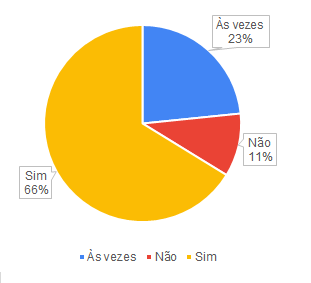
\includegraphics{images/Grafico-leitura-regulamentos.png}
    \caption{Você lê os regulamentos das hackathons que participa?}%pergunta 7
    \label{fig:le-regulamento}
\end{figure}


Foi questionado sobre o que o participante acha mais interessante ao ler o regulamento de uma hackathon. Essa foi uma pergunta facultativa, a qual recebemos 27 (vinte e sete respostas), algumas com duas ou mais propostas de tópicos, destrinchando-as foi totalizado 68 (sessenta e oito) tópicos. Por ser uma pergunta aberta, tivemos que agrupar os dados, pois o Google Forms não consegue agrupar em caso de divergência, muitas vezes mínima, com relação à grafia da palavra digitada. %Pergunta 8
Algumas ressalvas devem ser pontuadas, como a junção de propriedade industrial em propriedade intelectual, alguns critérios como "entender como funciona", "todos", "objetivos", foram tratados como generalidades.

\begin{figure}[H]
    \centering
    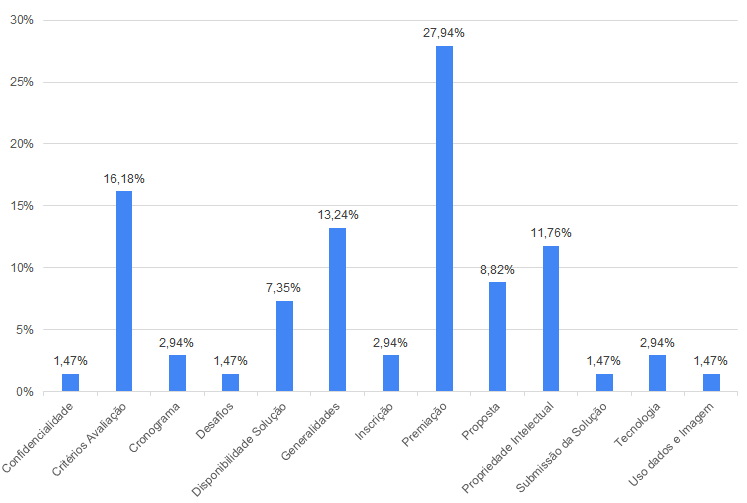
\includegraphics[width=0.8\textwidth]{images/topico-interessante.png}
    \caption{Qual tópico você acha interessante ao ler um regulamento de Hackathon?}% pergunta 8
    \label{fig:topico-interessante}
\end{figure}


Foi proposto um ranking dentre cinco tópicos aos participantes, onde eles teriam que categorizar o quanto eles consideram os seguintes tópicos ao ler o regulamento de uma hackathon do mais relevante ao menos relevante: Programação do Evento, direitos à Propriedade Intelectual, premiação,formação da equipe, premiação e critério de avaliação. Conforme pode ser visto na \autoref{fig:ranking}. %pergunta 9

\begin{figure}[H]
    \centering
    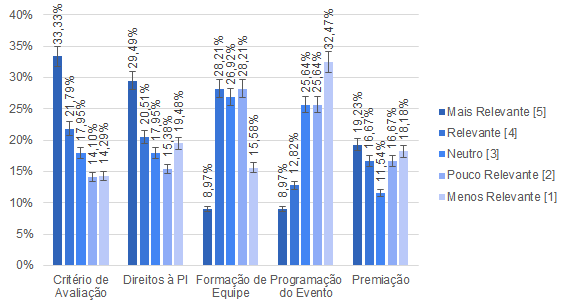
\includegraphics[width=0.8\textwidth]{images/ranking.png}% talvez tenha q melhorar a figura
    \caption{De 1 a 5, sendo 5 o MAIS relevante e 1 o MENOS relevante, o quão relevante você considera os seguintes tópicos ao ler o regulamento de uma Hackathon?}
    \label{fig:ranking}
\end{figure}%pergunta 9



Foi perguntado o quão importante é para o participante, no regulamento, o tópico de propriedade intelectual. Conforme pode ser visto o gráfico contido na \autoref{fig:importancia}.

\begin{figure}[H]
    \centering
    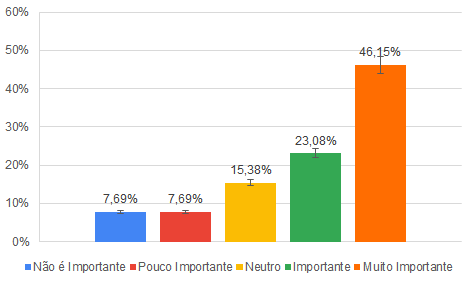
\includegraphics{images/importante.png}
    \caption{O quão importante é pra você no Regulamento o tópico de Propriedade Intelectual?}
    \label{fig:importancia}
\end{figure}


A pergunta 11 do questionário tentou avaliar a clareza dos regulamentos quanto à quem fica os direitos à propriedade intelectual do conteúdo feito pelo participante nas hackathons. De acordo com a \autoref{fig:clareza}

\begin{figure}[H]
    \centering
    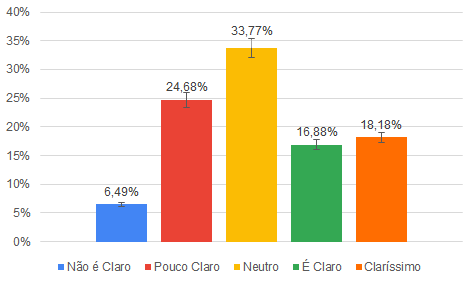
\includegraphics{images/clareza.png}
    \caption{O regulamento é sempre claro para quem fica os direitos à propriedade intelectual do conteúdo feito por você naquele evento?}
    \label{fig:clareza}
\end{figure}

A 12ª (décima segunda) pergunta do questionário foi pedido ao participante para afirmar se geralmente cedem os seus direitos à Propriedade Intelectual numa hackathon. 53,6\% afirmaram que cedem sim, os seus direitos, os outros 45,4\% afirmaram que não cedem os direitos.

Objetivamente foi perguntado se o participante venderia o protótipo da solução desenvolvida no hackathon. Obtivemos massivamente 90\% afirmando que venderia a solução e apenas 10\% não venderia.

Relacionada à pergunta anterior, foram sugeridos valores pelo qual o participante venderia sua solução, conforme pode ser visto na \autoref{fig:valor-sugerido}

\begin{figure}[H]
    \centering
    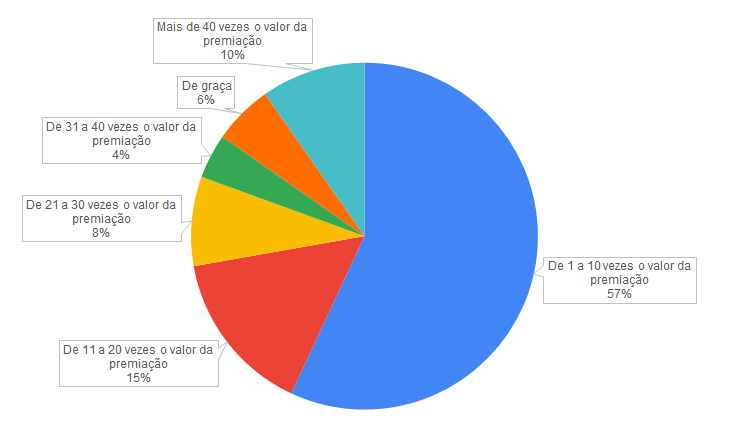
\includegraphics[width=0.7\textwidth]{images/Grafico-valor-venda-solucao.png}
    \caption{Venderia o protótipo da solução desenvolvida no hackathon?}
    \label{fig:valor-sugerido}
\end{figure}

%   pergunta 15
Também foi perguntado se o participante deixaria de participar de uma hackathon caso não ficassem com os direitos à propriedade intelectual. Em sua maioria, 55,9\% afirmam que deixaria de participar do evento caso o direito não pertencesse à pessoa. Os outros 44,1\% pessoas não deixariam de participar do evento.

Dentre os participantes, 49,35\% afirmaram que já abriu mão de propriedade intelectual em algum hackathon, enquanto 50,65\% afirmam não terem aberto mão. %pergunta 16

Os participante indagaram sobre o quanto a PI é respeitada nos eventos, assim como o interesse em saber ou entender sobre os direitos que eles têm sobre a PI conforme podem ser vistos nas \autoref{fig:respeito} e \autoref{fig:interessante-entender} abaixo. %pergunta 17 e 18

\begin{figure}[H]
    \centering
    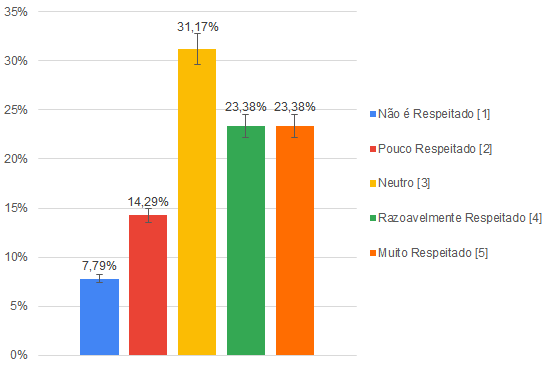
\includegraphics[width=0.8\textwidth]{images/PIrespeitada.png}
    \caption{Nos eventos em que participou, o quanto você sente que seu direito à propriedade intelectual é respeitado?}
    \label{fig:respeito}
\end{figure}



\begin{figure}[H]
    \centering
    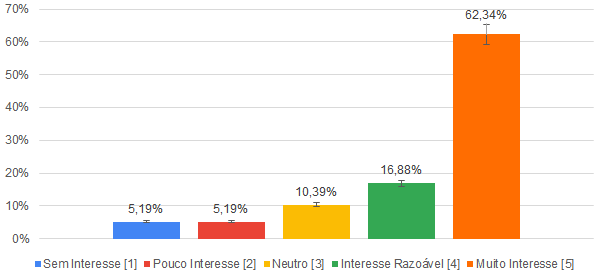
\includegraphics[width=0.8\textwidth]{images/interesseAprender.png}
    \caption{O quão interessante você acha saber/entender sobre a propriedade intelectual e seus direitos sobre ela?}
    \label{fig:interessante-entender}
\end{figure}



A penúltima pergunta indaga sobre a confiança em ceder os códigos-fonte após o evento para a empresa organizadora, onde 49,35\% afirmam não confiarem, enquanto 50,65\% asseguram confiança em ceder os códigos-fonte à empresa organizadora após o evento.
